\documentclass[usenames, dvipsnames, aspectratio=75]{beamer}
\usepackage[utf8]{inputenc}
\usepackage[T1]{fontenc}
\usepackage[ngerman]{babel}
\usepackage[defaultfam, regular]{montserrat}
\usepackage[german=guillemets]{csquotes}
\usepackage{hyperref}
    \hypersetup{colorlinks=true, citecolor=purple, filecolor=black, linkcolor=TealBlue, urlcolor=blue}
\usepackage{latexsym,multicol,booktabs,miama}
\usepackage{setspace}
\usepackage{xcolor}
\usepackage{tikz}
\usetikzlibrary{shapes.geometric, arrows}
\tikzstyle{task} = [rectangle, rounded corners, text centered, draw=black,
    minimum width=4cm, minimum height=1.5cm]
\usepackage{amssymb,amsfonts,amsmath,amsthm,mathrsfs,mathptmx} 
\usepackage{graphicx,pstricks,listings,stackengine}
\usepackage[figurename=Fig., tablename=Tab., font=footnotesize]{caption}
\usepackage[backend=biber,bibencoding=utf8,urldateusetime=true,style=alphabetic,sorting=nyt,natbib=true]{biblatex}
\usepackage{tcolorbox} % For creating colored boxes
\usepackage{svg}
\addbibresource{assets/refs.bib}

\setcounter{biburllcpenalty}{7500}
\setcounter{biburlucpenalty}{8000}

\setbeamertemplate{bibliography item}{\insertbiblabel}

\usepackage{todonotes}
\newcommand{\newtodo}[1]{\vspace{.75em}\todo[inline,color=yellow]{#1}}
\setlength {\marginparwidth }{2cm}

\author{Jakob Engelbert Tomahogh}

\title[]{Sicherheitsanalyse durch Entwicklung eines Rogue Device zur Echtzeitmanipulation maritimer Steuerungssysteme}
\institute[]{
\inst{}
\footnotesize{Betreuer: \textit{M.Sc. Marvin Davieds}} \vspace*{.25em} \\
\footnotesize{Zweitgutachter: \textit{Prof. Dr. rer. nat. Clemens H. Cap}}
}
\date{14.02.2025}

\usepackage{assets/EXTRAS}

\def\cmd#1{\texttt{\color[RGB]{0, 0, 139}\footnotesize $\backslash$#1}}
\def\env#1{\texttt{\color[RGB]{0, 0, 139}\footnotesize #1}}

\lstdefinestyle{texstyle}{
    language=[LaTeX]TeX,
    basicstyle=\ttfamily\footnotesize,
    keywordstyle={\bfseries\color[RGB]{0, 0, 180}},
    keywordstyle=[2]{\slshape\color[RGB]{225, 140, 30}},
    morekeywords=[2]{,itemize, enumerate, equation, table, tabular},
    stringstyle=\color[RGB]{50, 50, 50},
    numbers=left,
    numberstyle=\footnotesize\color{gray},
    rulesepcolor=\color{red!20!green!20!blue!20},
    frame=shadowbox
}

\begin{document}

\begin{frame}
    \vspace*{.25em}
    \begin{figure}[htpb]
        \centering
        
\includegraphics[width=0.55\linewidth]{assets/logo_uni_rostock.jpg}
    \end{figure}
    \vspace*{-1.5em}
    \titlepage
\end{frame}

\section{Einführung}

\subsection{Motivation}

\begin{frame}{Motivation}
    \begin{itemize}
        \item Sicherheit wurde in maritimen Systemen vernachlässigt
        \item Kommunikationssysteme sind anfällig für Angriffe
        \item Angriff auf Steuerungssysteme könnte katastrophale Folgen haben
        \item physischer Zugriff bei Passagierschiffen möglich
    \end{itemize}
\end{frame}

\subsection{Zielsetzung}
    \begin{frame}{Zielsetzung}
        \begin{itemize}
            \item Steuerung eines Schiffes durch ein Spielecontroller
            \item Rogue Device als Schnittstelle zwischen Controller und Schiff
            \item Unbemerkte Manipulation der Steuerung
        \end{itemize}
    \end{frame}

    \begin{frame}{Zielsetzung}
        \begin{itemize}
            \item Machbarkeit eines solchen Angriffs soll gezeigt werden
            \item Aufmerksamkeit auf Sicherheitslücken in maritimen Systemen lenken
            \item Sicherheitslücken sollen durch Steueurung mit Spielecontroller veranschaulicht werden
            \item Betrachtung möglicher Gegenmaßnahmen
        \end{itemize}
    \end{frame}
% ---------------------------------------------------------------------------

\section{Grundlagen}

\subsection{Schiffstechnik}
\begin{frame}{Schiffstechnik}
    \begin{figure}
        \centering
        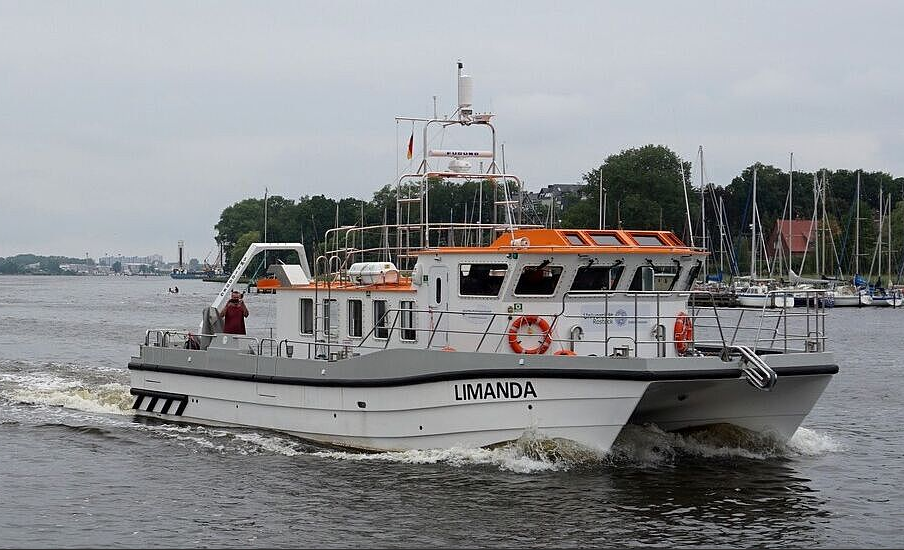
\includegraphics[width=0.6\linewidth]{assets/limanda.png}
        \caption{Forschungsschiff Limanda}
    \end{figure}
    \begin{itemize}
        \item zweimotoriger Katermaran
        \item Länge: 15,73m 
        \item Breite: 6,16m
    \end{itemize}
\end{frame}

\begin{frame}{Schiffstechnik}
    \begin{figure}
        \centering
        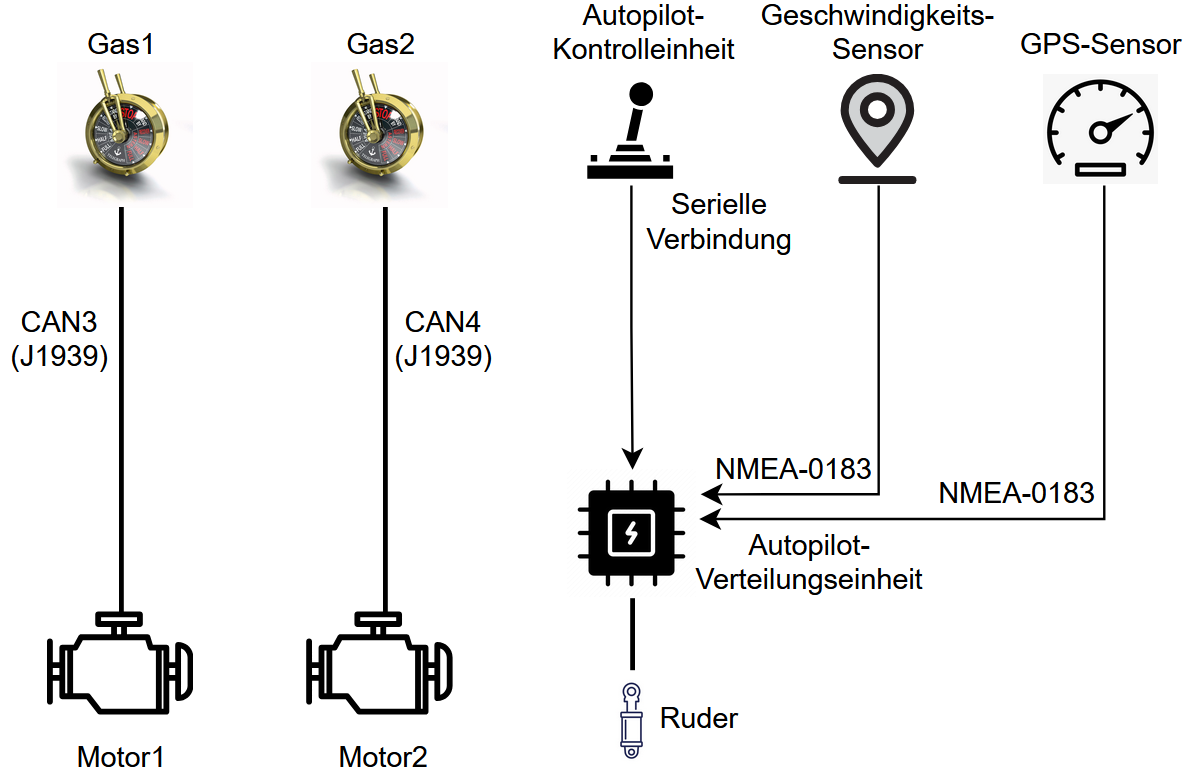
\includegraphics[width=1\linewidth]{assets/limandaSystem.png}
        \caption{Vereinfachter Aufbau des Systeme}
    \end{figure}
\end{frame}

\subsection{CAN-Bus}
\begin{frame}{CAN-Bus}
    \begin{itemize}
        \item serielle Netzwerktechnologie, bei dem mehrere Geräte miteinander kommunizieren können
        \item ermöglicht effiziente Kommunikation zwischen Steuergeräten
        \item alle Geräte sind gleichberechtigt
        \item Nachrichten werden nach Broadcast-Prinzip übertragen
        \item Kommunikation auf dem CAN-Bus ist unverschlüsselt
    \end{itemize}
\end{frame}

\begin{frame}{CAN-Bus Nachricht}
    \begin{figure}
        \centering
        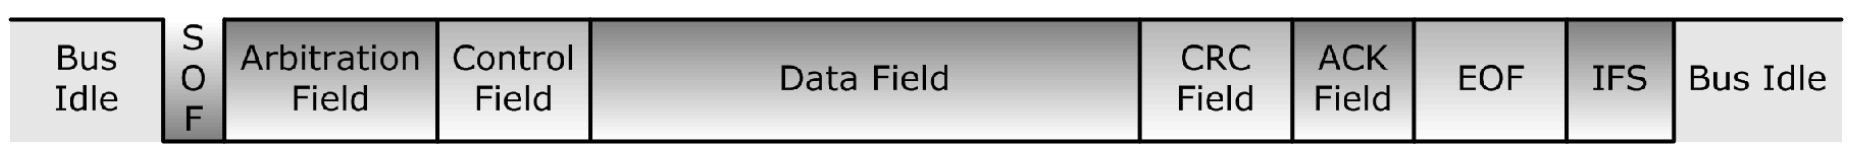
\includegraphics[width=0.9\linewidth]{assets/canMessage.png}
        \caption{Aufbau einer CAN-Bus Nachricht}
    \end{figure}
    \begin{itemize}
        \item \textbf{SOF}: Start of Frame
        \item \textbf{Arbitration Field}: Nachrichten-ID und Remote Transmission Request
        \item \textbf{Control Field}: Datenlänge
        \item \textbf{Data Field}: Nutzdaten
        \item \textbf{CRC Field}: Prüfsumme
        \item \textbf{EOF}: End of Frame
        \item \textbf{IFS}: Interframe Space, Pause zwischen Nachrichten
    \end{itemize}
\end{frame}

\begin{frame}{J1939}
    \begin{itemize}
        \item Standard für die Kommunikation auf dem CAN-Bus
        \item Nutzt 29 Bit Extended CAN Identifier
        \item ermöglicht Knotenadressierung
    \end{itemize}
\end{frame}

\begin{frame}{J1939}
    \begin{figure}
        \centering
        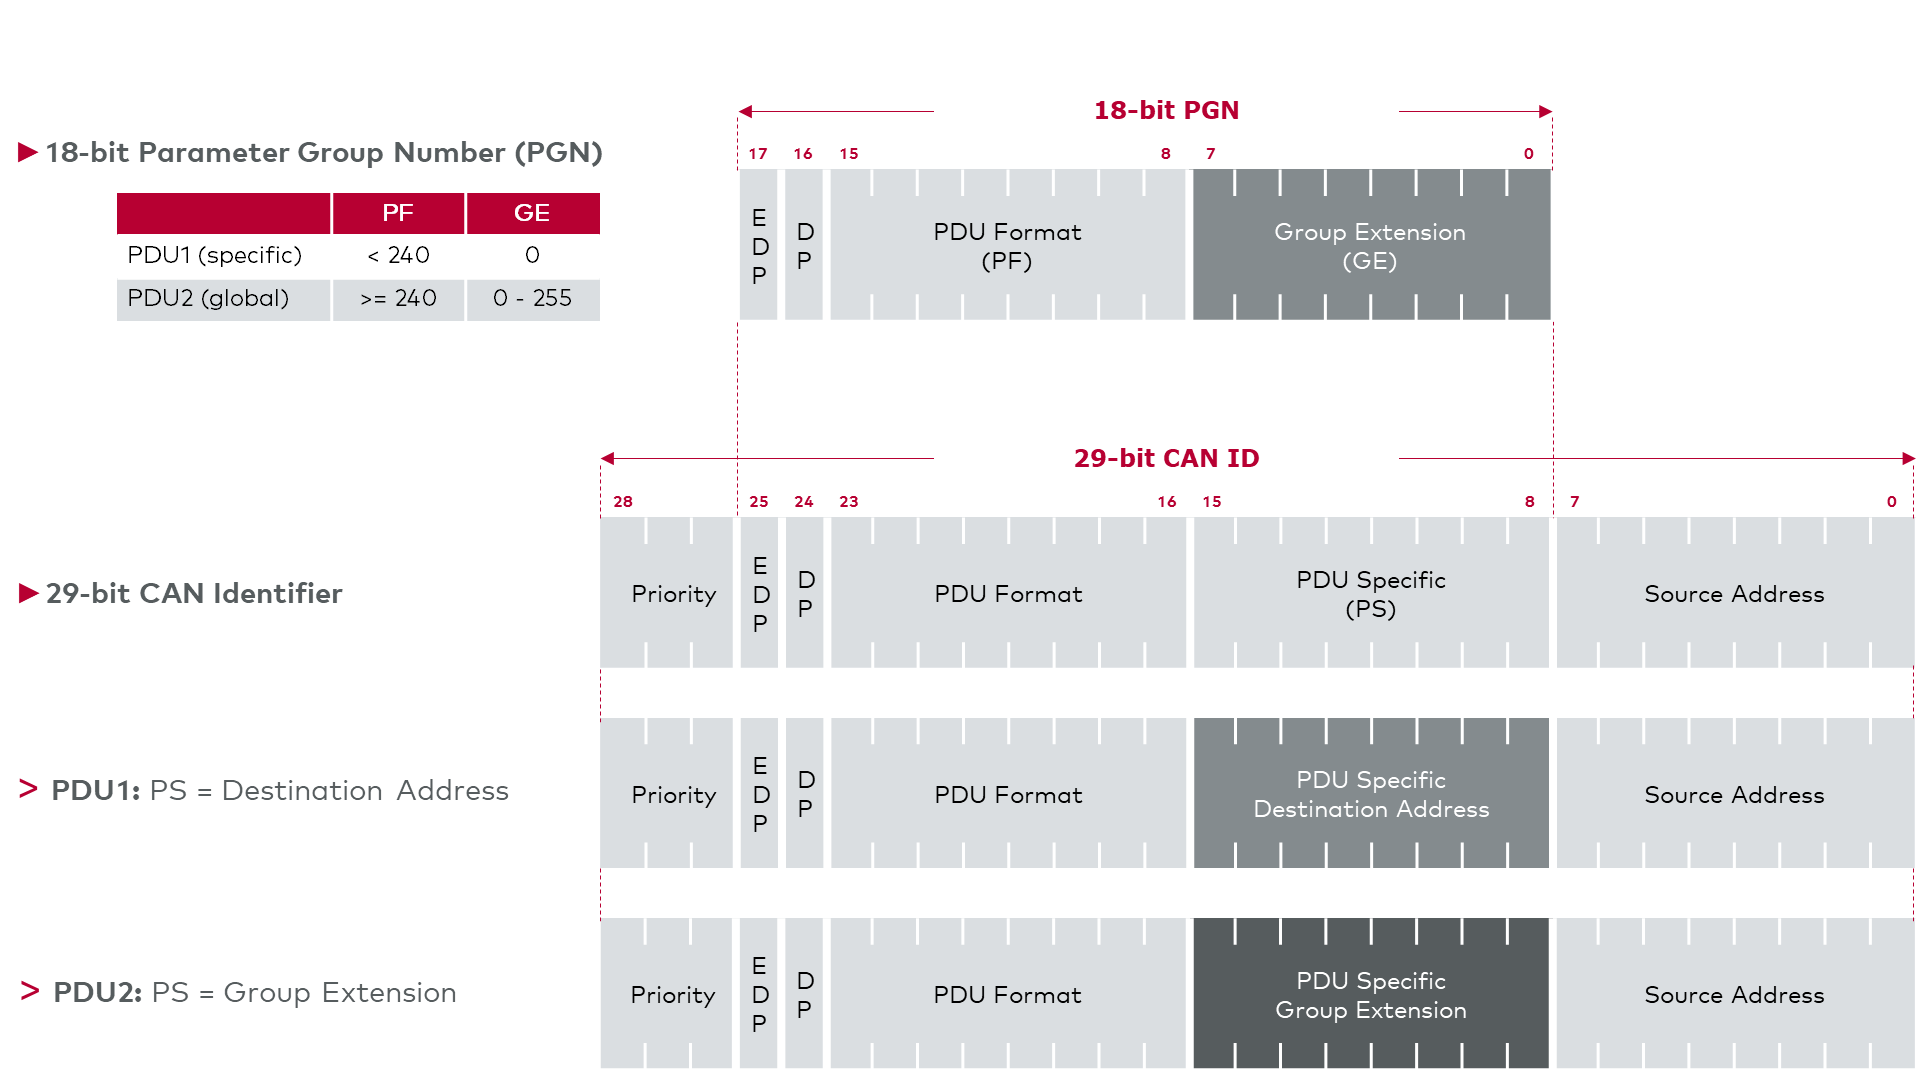
\includegraphics[width=1\linewidth]{assets/j1939id.png}
        \tiny{Quelle: \url{https://www.vector.com/de/de/know-how/protokolle/sae-j1939/}}
        \caption{J1939 Nachrichten-ID}
    \end{figure}
\end{frame}

% ---------------------------------------------------------------------------

\section{Konzept}
\begin{frame}{Konzept}
    \begin{itemize}
        \item Xbox Controller als Eingabegerät
        \item Raspberry Pi 5 als Rogue Device
        \item Anbindung des Raspberry Pi an den CAN-Bus
        \item Übersetzung der Controllereingaben in CAN-Bus Nachrichten auf Rogue Device
    \end{itemize}
\end{frame}

\begin{frame}{Konzept}
    \begin{figure}
        \begin{itemize}
            \item Unterbindung der originalen Steuerung
            \item Reaktion auf Nachrichten der Gashebel
            \item Rückmeldung der derzeitigen Eingaben des Xbox-Controllers
            \item Rudersteuerung über Autopiloten
        \end{itemize}
    \end{figure}
\end{frame}

\section{derzeitiger Stand}

\begin{frame}{derzeitiger Stand}
    \begin{itemize}
        \item Raspberry Pi mit Raspberry Pi OS
        \item Programmierung in Python
        \item Bedienungskonzept des Xbox-Controllers
    \end{itemize}
\end{frame}

\begin{frame}{derzeitiger Stand}
    \begin{figure}
        \centering
        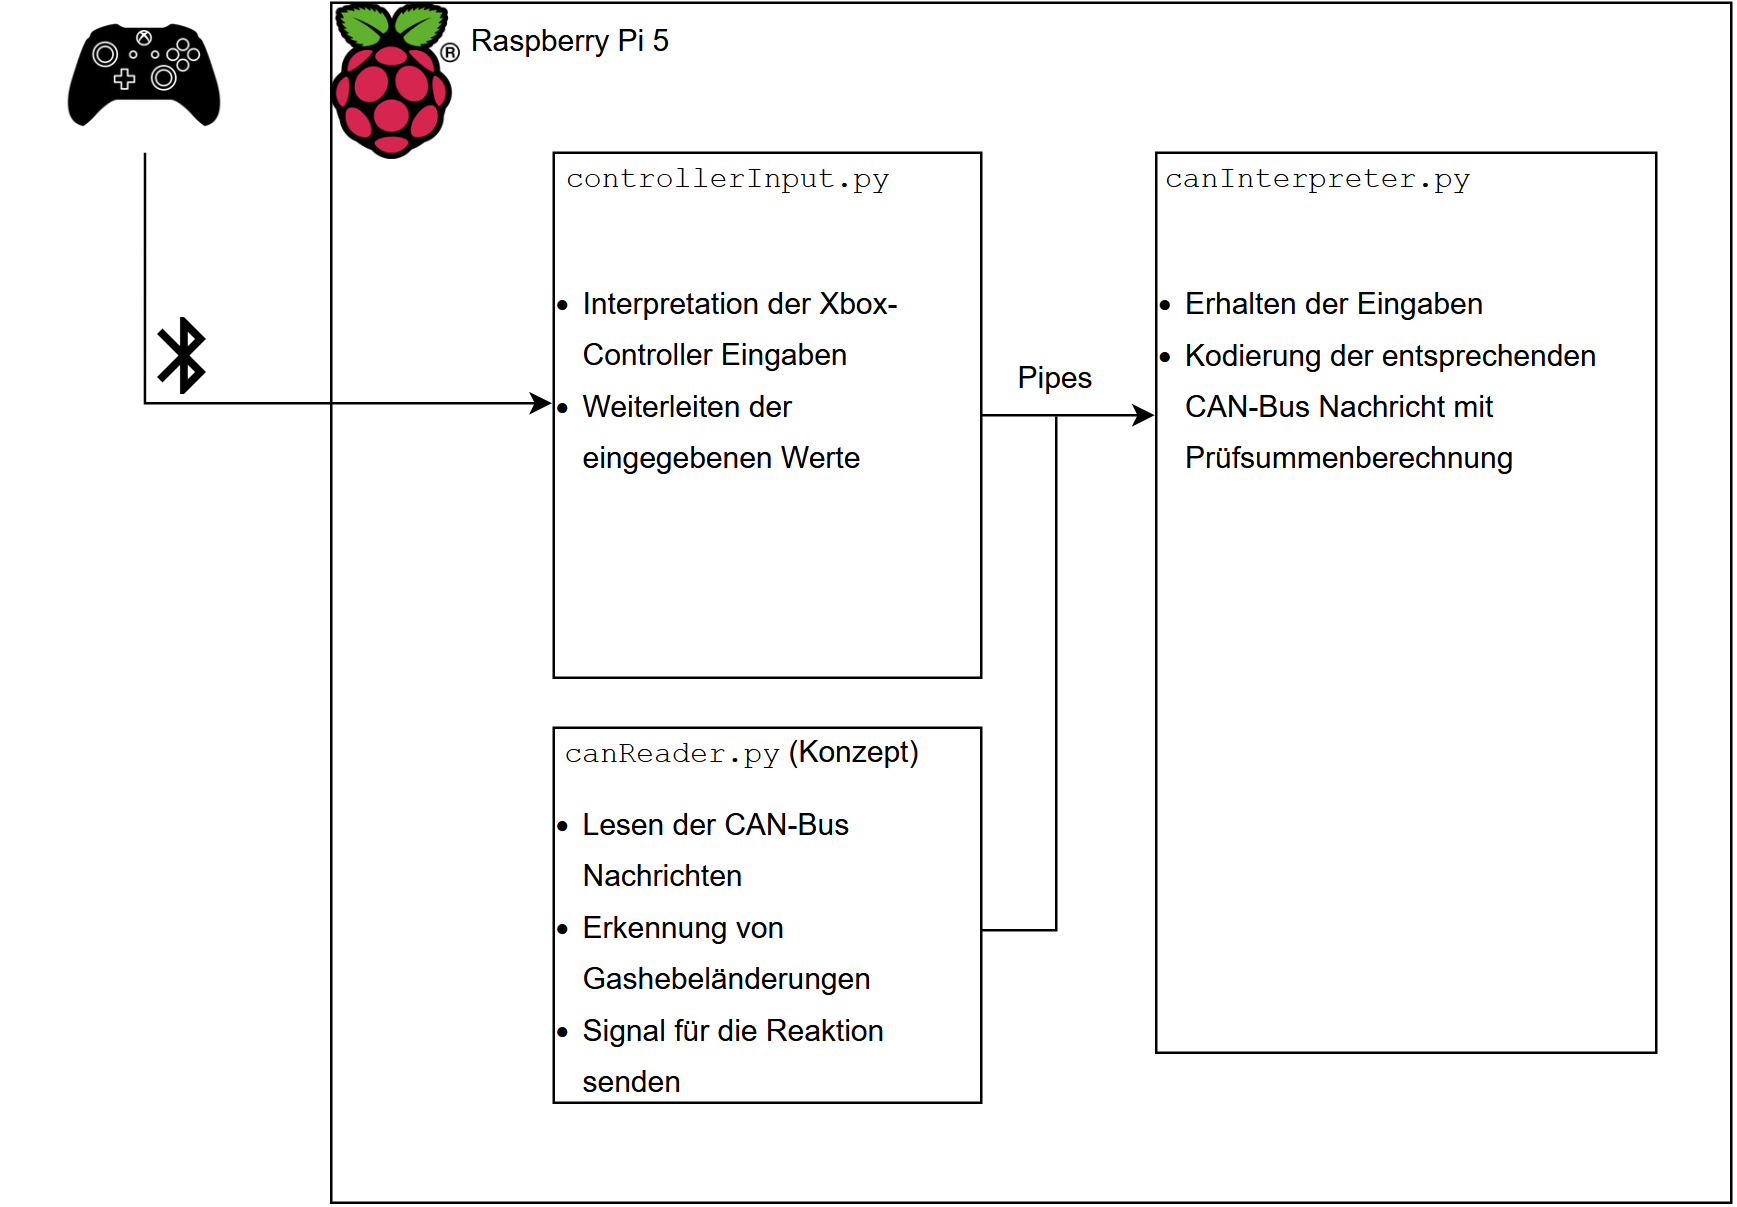
\includegraphics[width=0.85\linewidth]{assets/piKonzept.png}
        \caption{Programmstruktur auf dem Raspberry Pi} 
    \end{figure}
\end{frame}

\begin{frame}{derzeitiger Stand}
    \begin{itemize}
        \item Aufbau eines CAN-Bus Netzwerks mit UCAN (USB-zu-CAN Adapter)
        \item Kodieren der Eingaben in CAN-Bus Nachrichten \begin{itemize}
            \item cantools
            \item DBC-Datei
        \end{itemize}
    \end{itemize}   
\end{frame}

\begin{frame}{DBC-Datei}
    \begin{figure}
        \centering
        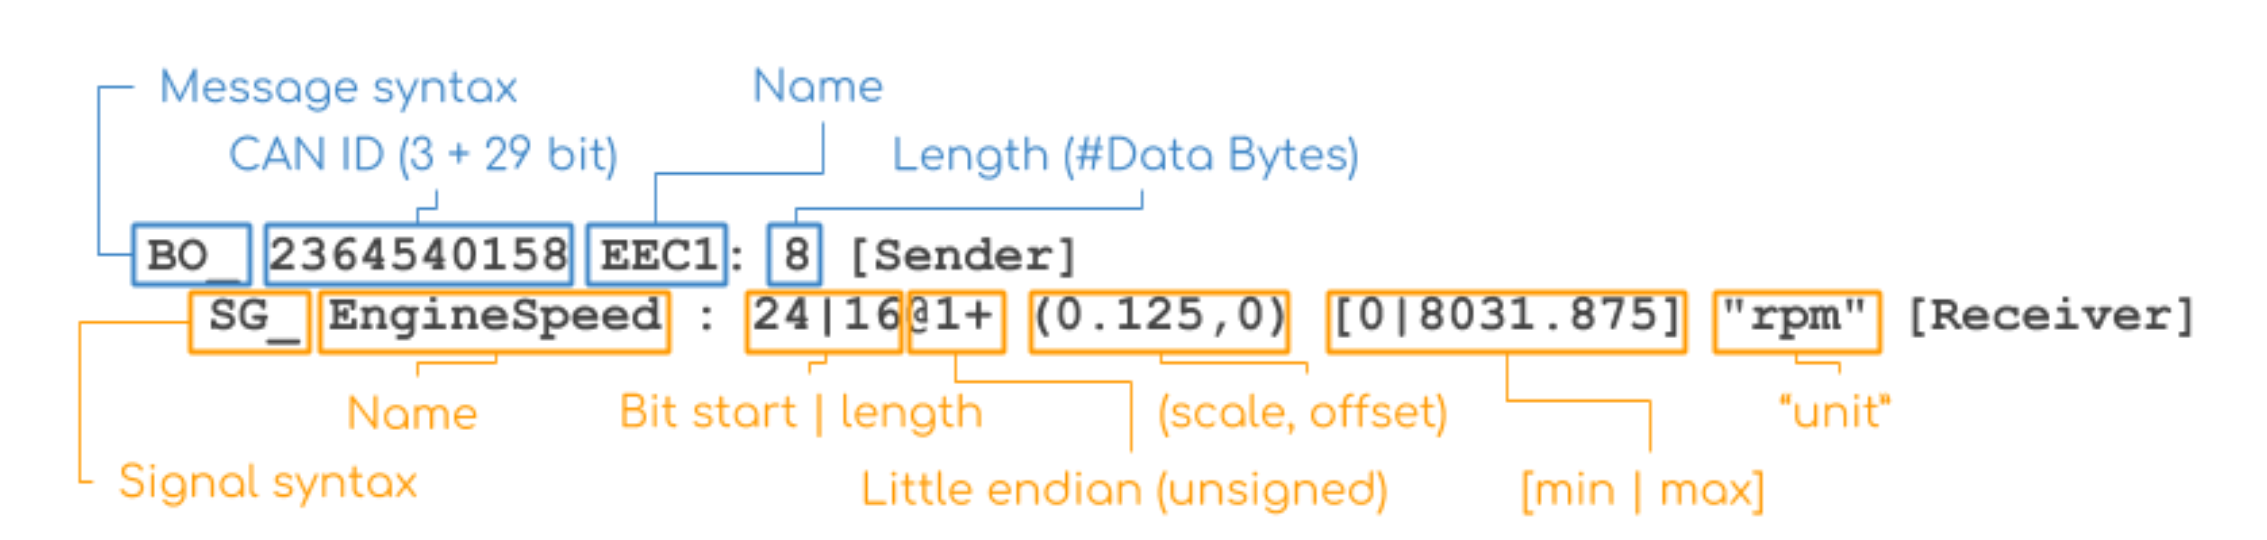
\includegraphics[width=1\linewidth]{assets/CAN-DBC-File-Format-Explained-Intro-Basics_2.png}
        \caption{Auszug einer Beispiel DBC-Datei}
    \end{figure}
\end{frame}

\begin{frame}{derzeitiger Stand}
    \begin{itemize}
        \item Anhand der DBC-Datei einzelne Signale mit validen Werten erstellt
        \item Frame-ID der DBC-Datei entnommen
        \item Prüfsumme mit Nachrichten-ID, ersten 7 Bytes und Nachrichtenzähler berechnet
        \item Daraus CAN-Bus Nachricht erstellt
    \end{itemize}
    
\end{frame}


\section{Ausblick}
\begin{frame}{Ausblick}
    \begin{figure}
        \centering
        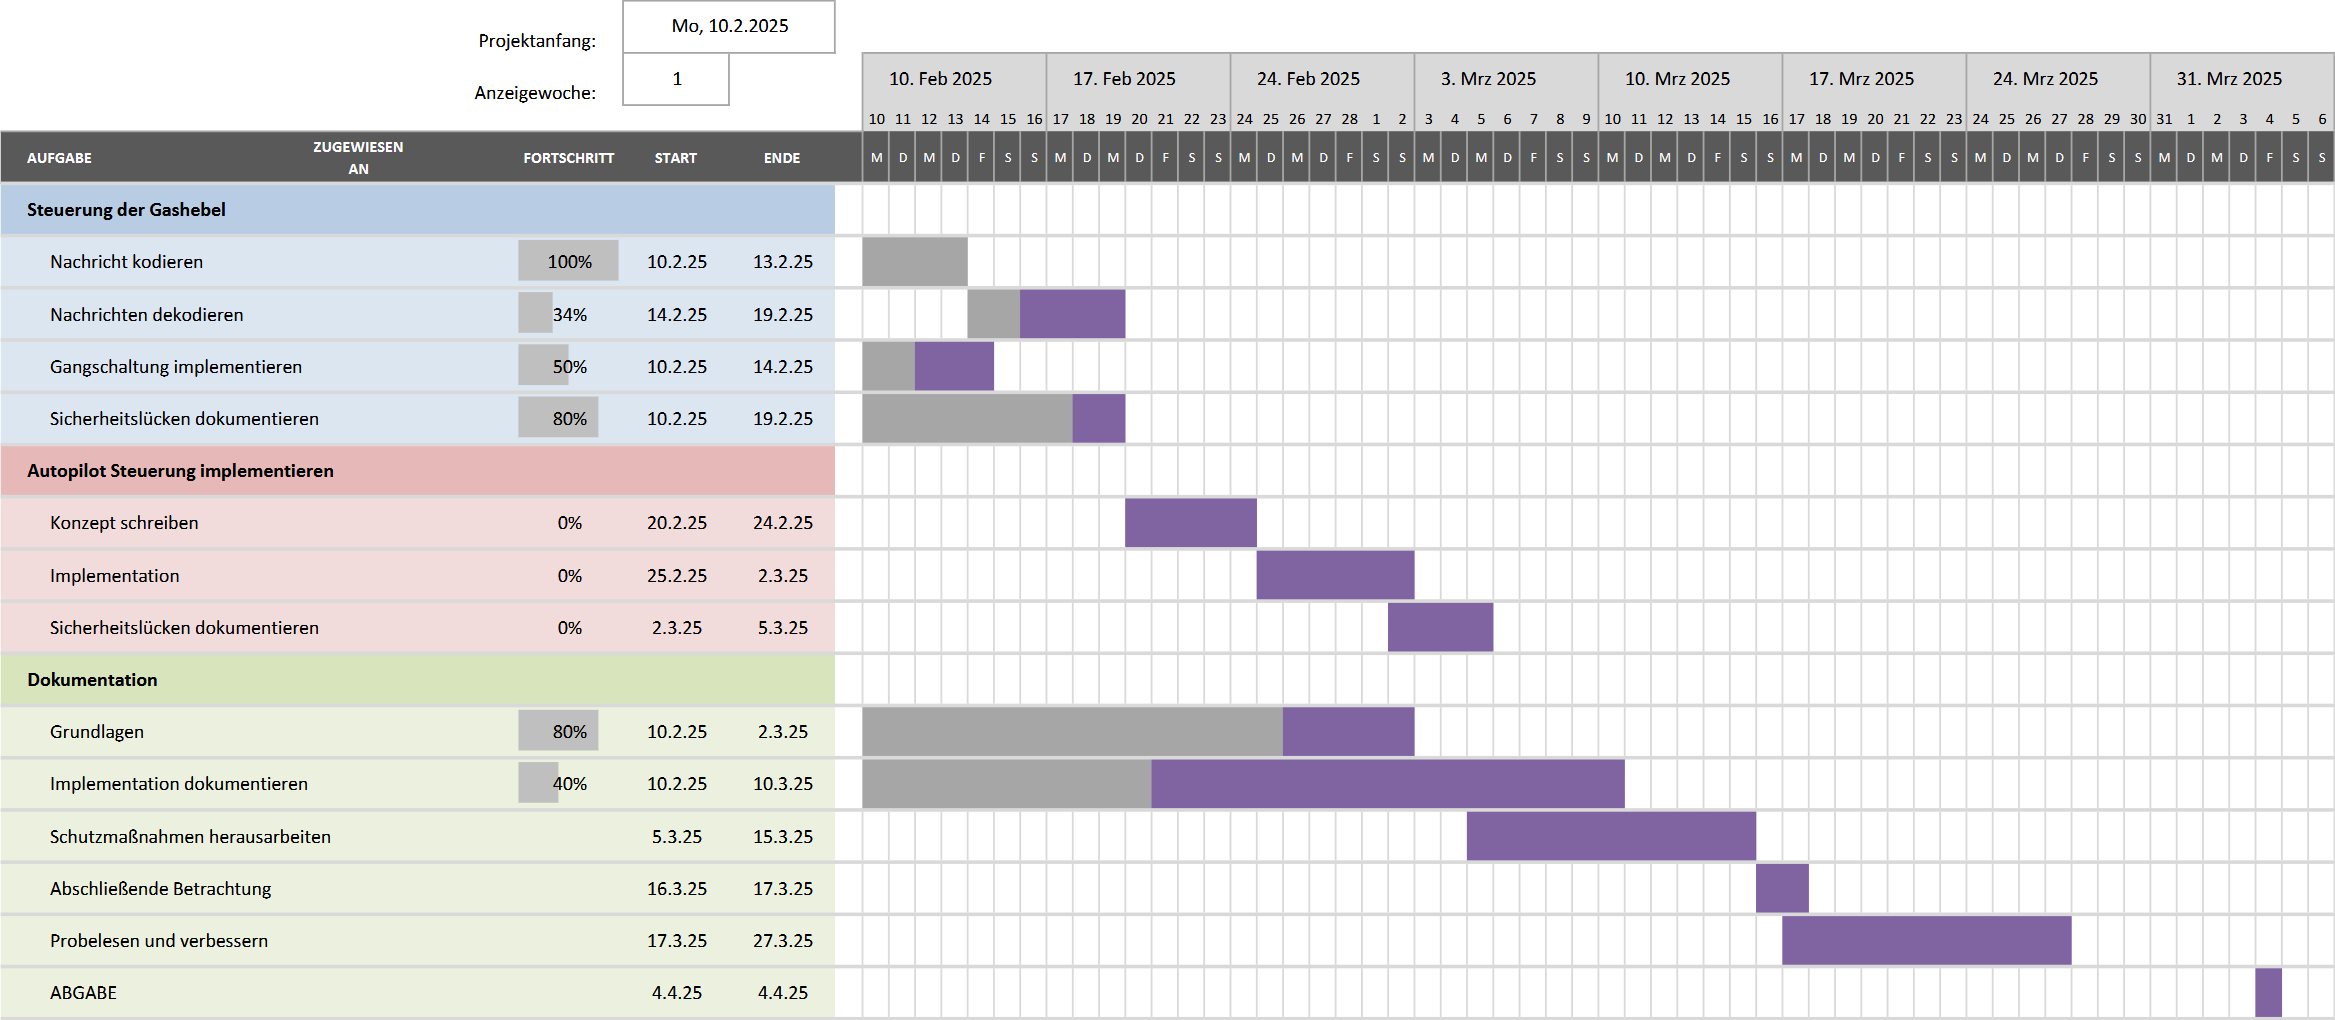
\includegraphics[width=1\linewidth]{assets/Zeitplan.png}
        \caption{Zeitplan}
    \end{figure}
\end{frame}

% ---------------------------------------------------------------------------

\end{document} 

